\documentclass[border=6pt]{standalone}
\usepackage{amsmath,amssymb}
\usepackage{xcolor}
\usepackage{tikz}
\usepackage{pgfplots}
\pgfplotsset{compat=1.17}
\usetikzlibrary{arrows.meta,positioning,calc}
\definecolor{cvviolet}{HTML}{4A3AA7}
\definecolor{cvblue}{HTML}{2A78D6}
\definecolor{cvaqua}{HTML}{1BAF7A}
\definecolor{ink}{HTML}{0B0B0B}
\definecolor{inks}{HTML}{52514E}
\definecolor{panel}{HTML}{F4F3EF}
\begin{document}
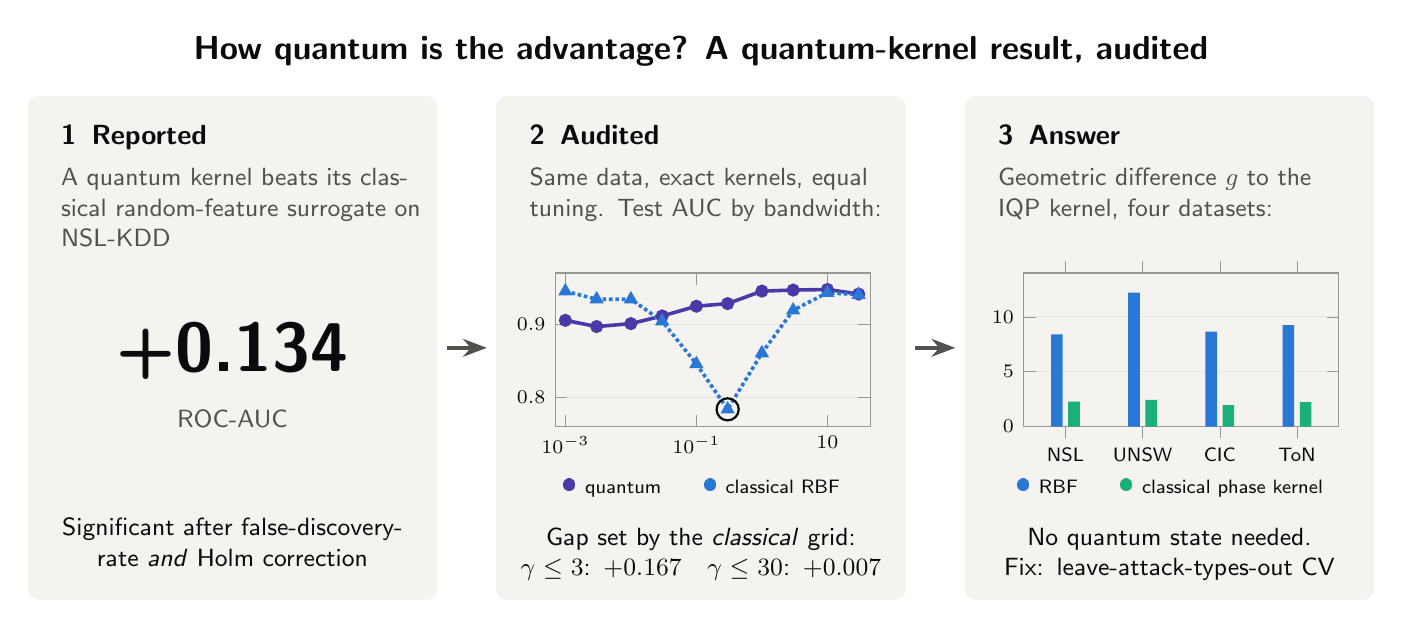
\begin{tikzpicture}[font=\sffamily\small, text=ink]
  \def\W{5.2} \def\H{6.4} \def\G{0.75}
  \foreach \x in {0, 1, 2} {
    \fill[panel, rounded corners=4pt] ({\x*(\W+\G)},0) rectangle ++(\W,\H);
  }
  \foreach \x in {1, 2} {
    \draw[-{Stealth[length=3mm]}, line width=1.4pt, inks]
      ({\x*(\W+\G)-\G+0.12},{\H/2}) -- ({\x*(\W+\G)-0.12},{\H/2});
  }
  \node[font=\sffamily\bfseries\large, anchor=south] at ({(3*\W+2*\G)/2},{\H+0.25})
    {How quantum is the advantage? A quantum-kernel result, audited};

  % -------- panel 1: the reported result ---------------------------------
  \begin{scope}[shift={(0,0)}]
    \node[anchor=north west, font=\sffamily\bfseries] at (0.3,\H-0.25) {1\enspace Reported};
    \node[anchor=north west, text width=4.6cm, text=inks] at (0.3,\H-0.8)
      {A quantum kernel beats its classical random-feature surrogate on NSL-KDD};
    \node[font=\sffamily\bfseries\fontsize{30}{32}\selectfont] at (\W/2,3.15) {+0.134};
    \node[text=inks] at (\W/2,2.3) {ROC-AUC};
    \node[anchor=south, text width=4.6cm, align=center] at (\W/2,0.3)
      {Significant after false-discovery-rate \emph{and} Holm correction};
  \end{scope}

  % -------- panel 2: the audit ---------------------------------------------
  \begin{scope}[shift={(\W+\G,0)}]
    \node[anchor=north west, font=\sffamily\bfseries] at (0.3,\H-0.25) {2\enspace Audited};
    \node[anchor=north west, text width=4.6cm, text=inks] at (0.3,\H-0.8)
      {Same data, exact kernels, equal tuning. Test AUC by bandwidth:};
    \begin{axis}[at={(0.75cm,2.2cm)}, anchor=south west, scale only axis,
        width=4.0cm, height=1.95cm, xmode=log, xmin=0.0007, xmax=45, xminorticks=false,
        ymin=0.76, ymax=0.97, xtick={0.001,0.1,10}, xticklabels={$10^{-3}$,$10^{-1}$,$10$},
        ytick={0.8,0.9}, tick label style={font=\sffamily\scriptsize},
        axis line style={inks!60}, tick style={inks!60}, ymajorgrids, grid style={inks!15},
        every axis plot/.append style={line width=1.3pt, mark size=1.7pt}]
      \addplot[cvviolet, mark=*] coordinates
        {(0.001,0.9053)(0.003,0.8968)(0.01,0.9008)(0.03,0.9113)(0.1,0.9246)(0.3,0.9282)(1,0.9453)(3,0.9467)(10,0.9475)(30,0.9413)};
      \addplot[cvblue, densely dotted, mark=triangle*, mark options={solid}] coordinates
        {(0.001,0.9451)(0.003,0.9342)(0.01,0.9342)(0.03,0.9042)(0.1,0.8457)(0.3,0.7836)(1,0.8605)(3,0.9191)(10,0.9431)(30,0.9403)};
      \draw[ink, line width=0.8pt] (axis cs:0.3,0.7836) circle (4pt);
    \end{axis}
    \node[font=\sffamily\scriptsize] at (\W/2,1.42)
      {\textcolor{cvviolet}{\large\textbullet}\ quantum\qquad\textcolor{cvblue}{\large\textbullet}\ classical RBF};
    \node[anchor=south, text width=4.7cm, align=center] at (\W/2,0.12)
      {Gap set by the \emph{classical} grid:\\ $\gamma\le3$: $+0.167$\quad $\gamma\le30$: $+0.007$};
  \end{scope}

  % -------- panel 3: the answer ---------------------------------------------
  \begin{scope}[shift={(2*\W+2*\G,0)}]
    \node[anchor=north west, font=\sffamily\bfseries] at (0.3,\H-0.25) {3\enspace Answer};
    \node[anchor=north west, text width=4.6cm, text=inks] at (0.3,\H-0.8)
      {Geometric difference $g$ to the IQP kernel, four datasets:};
    \begin{axis}[at={(0.75cm,2.2cm)}, anchor=south west, scale only axis,
        width=4.0cm, height=1.95cm, ybar, bar width=4.2pt, ymin=0, ymax=14,
        symbolic x coords={NSL,UNSW,CIC,ToN}, xtick=data,
        ytick={0,5,10}, tick label style={font=\sffamily\scriptsize},
        enlarge x limits=0.18, axis line style={inks!60}, tick style={inks!60},
        ymajorgrids, grid style={inks!15}]
      \addplot[fill=cvblue, draw=none] coordinates {(NSL,8.41)(UNSW,12.21)(CIC,8.65)(ToN,9.25)};
      \addplot[fill=cvaqua, draw=none] coordinates {(NSL,2.27)(UNSW,2.44)(CIC,1.95)(ToN,2.23)};
    \end{axis}
    \node[font=\sffamily\scriptsize] at (\W/2,1.42)
      {\textcolor{cvblue}{\large\textbullet}\ RBF\qquad\textcolor{cvaqua}{\large\textbullet}\ classical phase kernel};
    \node[anchor=south, text width=4.7cm, align=center] at (\W/2,0.12)
      {No quantum state needed.\\ Fix: leave-attack-types-out CV};
  \end{scope}
\end{tikzpicture}
\end{document}
